\documentclass[aspectratio=1610]{beamer}

\usepackage[utf8]{inputenc}
\usepackage{graphicx}
\usepackage{amssymb}
\usepackage[export]{adjustbox}
\usetheme{Frankfurt}
\usefonttheme[onlymath]{serif}
\usepackage[super]{nth}
\graphicspath{{./Figures/}}
\usepackage{hyperref}
\hypersetup{
    colorlinks=true,
    linkcolor=athgold,
    filecolor=magenta,      
    urlcolor=cyan,
}
\usepackage{wasysym}
\definecolor{satinsheengold}{rgb}{.7608 .5569 0.0471}
\definecolor{athgold}{rgb}{0.8078, 0.7216, 0.5333}
\definecolor{dkgray}{rgb}{.2157, .2275, .2118}
\setbeamercolor{structure}{fg=satinsheengold}
\setbeamercolor{title}{fg=black}
\setbeamercolor{title in head/foot}{fg=black, bg=satinsheengold}
\setbeamercolor{author}{fg=dkgray}
\setbeamercolor{frametitle}{fg=black}
\setbeamercolor{author in head/foot}{fg=black, bg=satinsheengold}
\setbeamercolor{institute in head/foot}{bg=satinsheengold}
\setbeamercolor{date in head/foot}{bg=satinsheengold}
\setbeamercolor{section in foot}{fg=white, bg=dkgray}
\setbeamercolor{section in head}{fg = athgold, bg = black} 
\setbeamercolor{navigation symbols}{fg=gray}
\setbeamercolor{block title}{bg=athgold, fg = black}
\setbeamercolor{item projected}{fg=black}
\setbeamercolor{footlinecolor}{fg = black, bg = white}
\setbeamertemplate{blocks}[rounded][shadow=false]
\setbeamertemplate{enumerate items}[circle]
%\setbeamertemplate{footline}[frame number]
%Adding frame #s
\setbeamertemplate{navigation symbols}{%
    \usebeamerfont{footline}%
    \usebeamercolor[bg]{footline}%
    \hspace{1em}%
    %\insertframenumber/\inserttotalframenumber
}
\setbeamertemplate{footline}[text line]{%
  \begin{beamercolorbox}[wd=\paperwidth,ht=2.25ex,dp=1ex]{section in head}%
	\hspace{.5em} 	
 	\makebox[0pt][l]{\,\color{athgold}{\insertsection}}
 	 \hspace*{\fill}\insertshortauthor\hspace*{\fill}%
 	 \llap{\insertpagenumber\,/\,\insertpresentationendpage\,}	
 	 \hspace{.5em}
  \end{beamercolorbox}
}

\setbeamertemplate{headline}[text line]{%
  \begin{beamercolorbox}[wd=\paperwidth,ht=2.25ex,dp=1ex,center]{section in head}%
 BME 695 $|$ Numerical Methods
 %\inserttitle
  \end{beamercolorbox}
}


\title{Coding Assignment 3}
\author[Andrew Sivaprakasam]{Andrew Sivaprakasam}

\date{05/05/2021}

%Change this to section titles when you have a pres with multiple sections
\section{\insertshorttitle}
\begin{document}

\frame{\titlepage}

\section{Problem 1}

\begin{frame}
\frametitle{Problem 1 | Lotka-Volterra Model}
\textbf{\underline{Part 1: Questions from Biology Corner}}
\begin{enumerate}
\item \footnotesize{Over time, the grass becomes healthier/greener as rabbit population declines, since less rabbits are there to eat it. Rabbits get more populous with more abundant green grass. Wolves don't survive because the wolf population is so highly dependent on the rabbit population density that when the rabbit population decreases, the large number of wolves cannot survive/mate. 
\item In order to get a stable run for 1000+ iterations, the parameters need to be modified s.t. the wolves clear out just the right amount of rabbits as the grass gets eaten up. I did this by setting Rabbit repo age to \textbf{5}, the wolf repo age to \textbf{15} and wolf repo food level to \textbf{140}}.

\item For the above to work, forest size needed to be set at \textbf{huge}.

\vspace{1em}
\centering
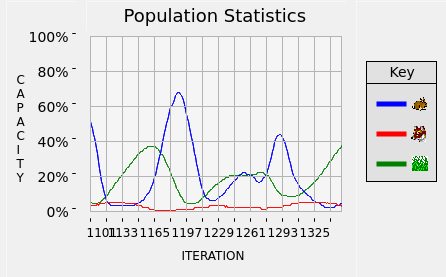
\includegraphics[width = .45\textwidth]{sim_1000} 
\end{enumerate}
\end{frame}


\begin{frame}
\frametitle{Problem 1 | Lotka-Volterra Model}

\end{frame}

\end{document}